\documentclass[12pt,letterpaper]{article}
\usepackage[utf8]{inputenc}
\usepackage{amsmath, amsfonts, amssymb}
\usepackage{graphicx}
\usepackage{geometry}
\usepackage{caption}
\usepackage{subcaption}
\usepackage{hyperref}

%% Packages setup
\geometry{
	verbose,
	letterpaper,
	tmargin=2cm,
	bmargin=2cm,
	lmargin=2cm,
	rmargin=2cm
    }

\hypersetup{
	bookmarksopen=true,
	colorlinks=true,
	linkcolor=blue,
	citecolor=blue,
	urlcolor=black,	
	linktoc=all,
	pdftitle={Dispersion in spring-mass lattices},
	pdfauthor={N. Guarin-Zapata},
	pdfkeywords={Dispersion, Phononic crystals, Vibrations, Wave propagation},
	pdfsubject={Dispersion in lattices},
	pdfpagemode=UseOutlines,
	pdfstartview=FitH
    }

\captionsetup{
    margin=20pt,
    font=small,
    labelfont=bf,
    labelsep=period
    }

%%
\author{Nicol\'as Guar\'in Zapata}
\title{\textbf{Dispersion relations for spring-mass lattices}}
\begin{document}
\maketitle

%% 
\section{Simple mass-spring lattice}
%Figure
\begin{figure}[h]
\centering
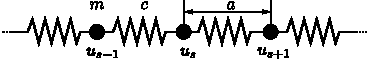
\includegraphics[height=1.5cm]{img/spring-mass.pdf} 
\caption{Simple mass-spring lattice.}
\end{figure}
\subsection{Direct formulation}
The force in the plane $s$ cause by the displacement of the plane $s+p$ is proportional to the difference $u_{s+p}-u_s$ of the displacements. For brevity we will consider only nearest-neighbor interactions, so $p=\pm 1$. The total force on $s$ comes from planes $s=\pm 1$:
\begin{equation}
F_s = c(u_{s+1}-u_s)+ c(u_{s-1}-u_s).
\end{equation}
The constant $c$ is the stiffness between nearest-neighbour planes and will differ for longitudinal and transverse waves.

The equation of motion of the plane $s$ is
\[ m  \ddot{u} = c(u_{s+1} + u_{s-1} -2 u_s), \]
assuming a harmonic time dependence $\exp(-i\omega t)$
\begin{equation}
-m\omega^2 u_s = c(u_{s+1} + u_{s-1} - 2u_s) \enspace .
\label{eq:single-spring-lattice}
\end{equation}
Due to the Bloch-periodicity condition
\[u_{s\pm 1} = u_s e^{\pm i ka}. \]
So (\ref{eq:single-spring-lattice}) is now
\[ -m \omega^2 u_s = c (u_s \exp(ika) + u_s \exp(-ika) - 2u_s) \]
and canceling $u_s$ from both sides, we have
\[ \omega^2 m = -c[ \exp(ika) + \exp(-ika) - 2 ] \enspace .\]
Using the identity $2\cos ka = \exp(ika) + \exp(-ika)$, and taking $\Omega^2 = \omega^2/\omega_0^2 = \omega^2 m/c$, we have the dispersion relation
\begin{equation}
\Omega^2 = 2 (1-\cos ka) \enspace .
\label{eq:simple-disp-relation}
\end{equation}
The boundary of the first Brillouin zone lies at $k=\pm \pi/a$. We show from (\ref{eq:simple-disp-relation}) that the slope of $\Omega$ versus $ka$ is zero at the zone boundary
\[ \frac{d\Omega^2}{d\, ka} = 2\sin ka=0\]
at $ka=\pm \pi$, $\sin ka = 0$.

By a trigonometric identity (\ref{eq:single-spring-lattice}) may be written as
\begin{equation}
\Omega^2 = 4 \sin^2 \frac{1}{2}ka, \qquad \omega = 2\left\vert \sin \frac{1}{2} ka\right\vert \enspace .
\end{equation}

\begin{figure}[h]
\centering
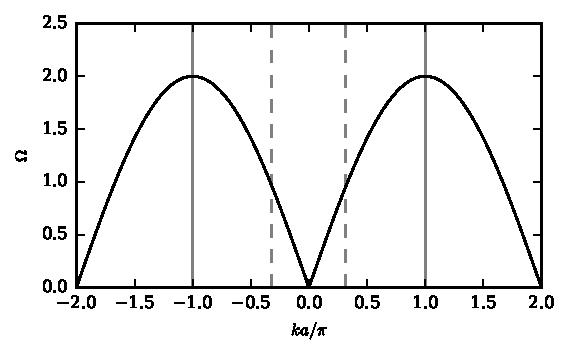
\includegraphics[height=8cm]{img/spring-mass-plot.pdf} 
\caption{Plot of $\Omega$ versus $ka$. The region of $ka<<1$ or $\lambda/a>>1$ corresponds to the continuum approximation; where $\Omega$ is directly proportional to $ka$ (and is enclosed between the dashed lines). The First Brillouin Zone is placed between $-1$ and $1$.}
\label{fig:spring-mass-dispersion}
\end{figure}

\subsection{Unit cell formulation}
This problem could also be solved taking a single cell and imposing the Bloch conditions after the assemblage process for the matrices. The force balance (in frequency domain) is
\begin{align*}
c(u_2 - u_1) &= -\frac{m}{2} \omega^2 u_1 \enspace ,\\
c(u_1 - u_2) &= -\frac{m}{2} \omega^2 u_2 \enspace ,
\end{align*}
we should take care since the total amount of mass in the cell should be consistent. That is why we choose each particle to have $m/2$. And this system could be expressed as
\begin{equation}
c\begin{bmatrix}
-1 & 1 \\ 
1 & -1
\end{bmatrix} \left\lbrace \mathbf{u} \right\rbrace =
-\frac{m\omega^2}{2}
\begin{bmatrix}
1 & 0 \\ 
0 & 1
\end{bmatrix} \left\lbrace \mathbf{u} \right\rbrace \enspace ,
\end{equation}
or, using $\Omega^2 = \omega^2 m/c$
multiplying the second row by $\exp(-ika)$ and the second column by its complex conjugate $\exp(ika)$ we get
\begin{equation*}
\begin{bmatrix}
-1 & e^{ika} \\ 
e^{-ika} & -1
\end{bmatrix} \left\lbrace \mathbf{u} \right\rbrace =
-\frac{\Omega^2}{2}\begin{bmatrix}
1 & 0 \\ 
0 & 1
\end{bmatrix} \left\lbrace \mathbf{u} \right\rbrace \enspace ,
\end{equation*}
adding the second row to first one, and then adding the second column to first one yields
\begin{equation*}
\begin{bmatrix}
e^{ika}+e^{-ika}-2 & e^{ika}-1 \\ 
e^{-ika}-1 & -1
\end{bmatrix} \left\lbrace \mathbf{u} \right\rbrace =
-\frac{\Omega^2}{2}\begin{bmatrix}
2 & 1 \\ 
1 & 1
\end{bmatrix} \left\lbrace \mathbf{u} \right\rbrace \enspace .
\end{equation*}
Now, were interested just in the reduced system, we delete the second row and column and get
\begin{equation}
\left[ e^{ika}+e^{-ika}-2 \right] = -\Omega^2 \enspace ,
\end{equation}
and this could be rewritten as
\begin{equation}
\Omega = 2\left\vert \sin \frac{1}{2} ka\right\vert \enspace ,
\end{equation}
which is the same result obtained before.

The phase speed is
\[v_p = \frac{\Omega}{ka} = \frac{2}{ka}\left\vert \sin \frac{1}{2} ka\right\vert \enspace ,\]
and the group speed
\[v_g \equiv \nabla_{ka}\Omega = \frac{d\Omega}{d\, ka} = \cos \left(\frac{1}{2} ka\right) \text{sign}\left[\sin \frac{1}{2} ka\right] \]

\begin{figure}[h]
\centering
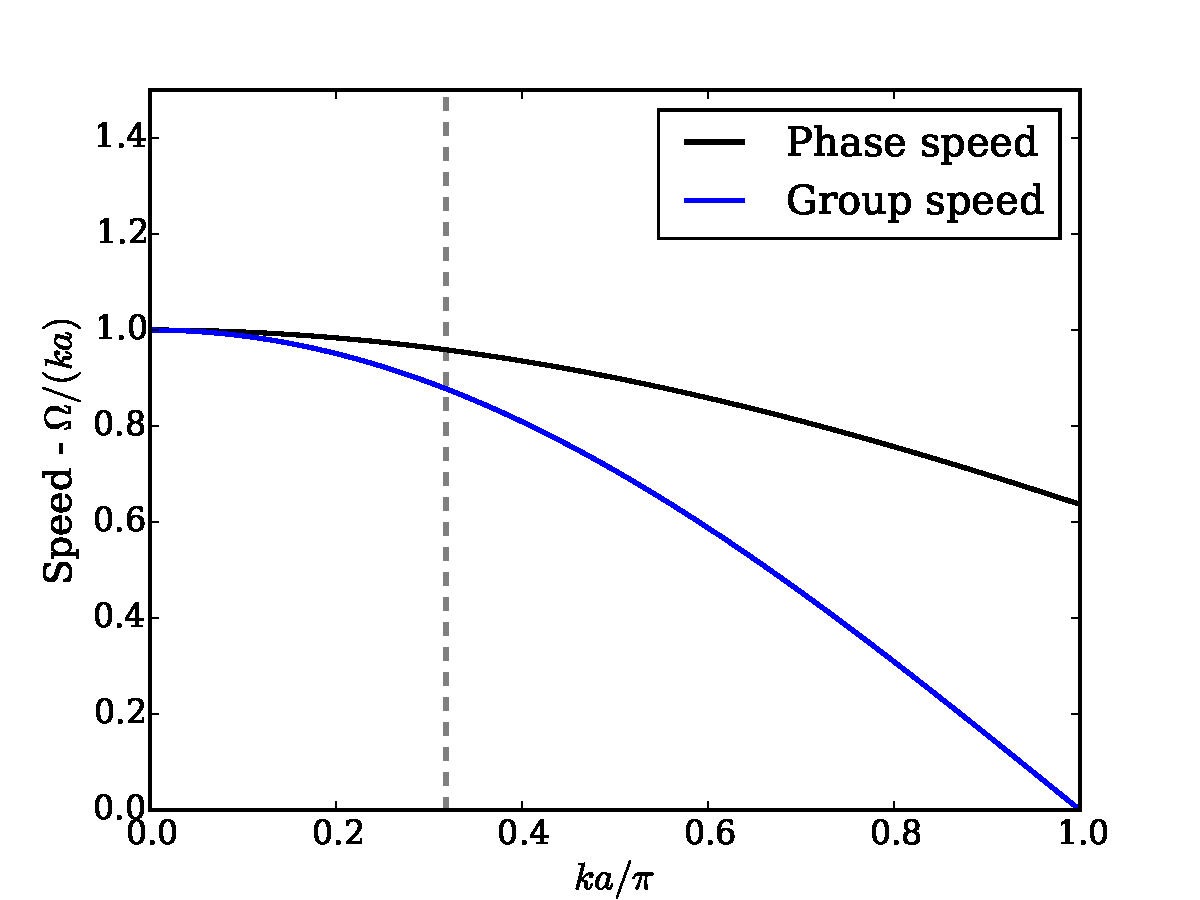
\includegraphics[height=8cm]{img/spring-mass-speeds.pdf} 
\caption{Plot of speed versus $ka$. The initial value is 1 and the approximation around 0 is constant speed.}
\label{fig:spring-mass-speed}
\end{figure}



\subsection{Finite case}
\begin{figure}[h]
\centering
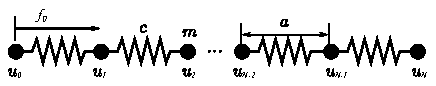
\includegraphics[width=4in]{img/spring-mass-finite.pdf} 
\caption{Finite simple mass-spring lattice.}\label{fig:spring-mass-finite}
\end{figure}
In practice, we cannot have infinite (periodic) repetition of unit cells, and, at some point, we need to truncate them to make them finite (Figure \ref{fig:spring-mass-finite}). When the number of unit cells increase, the behavior should get closer to the infinite case, and the presence of bandgaps could be inferred from the analysis of the response in frequency.

If we start from a single unit cell the equations of motion for harmonic force of frequency $\omega$ are given by
\begin{align*}
&-c(u_0 - u_1) + f_0 = -\omega^2 m u_0\\
&-c(u_1 - u_0) = -\omega^2 m u_1 \enspace ,
\end{align*}
or
\begin{equation}
\begin{bmatrix}
-1 + \Omega^2 & 1 \\ 
1 & -1 + \Omega^2
\end{bmatrix}
\begin{Bmatrix}
u_0 \\ 
u_1
\end{Bmatrix} =
\begin{Bmatrix}
-\hat{f}_0 \\ 
0
\end{Bmatrix} \enspace , 
\label{eq:1_cell_finite}
\end{equation}
where we normalized the equation.  $\Omega^2 = \omega^2/\omega_0^2 = \omega^2 m/c$ and $\hat{f}_0 = f_0/c$. And the solutions for this system of equations is
\begin{align*}
u_0 &= \frac{\hat{f}_0(1 - \Omega^2)}{\Omega^2(\Omega^2 - 2)}\\
u_1 &= \frac{\hat{f}_0}{\Omega^2(\Omega^2 - 2)} \enspace .
\end{align*}
We are interested in the response of the last mass with respect to the force impinged in the first one, i.e.
\begin{equation}
\frac{u_1}{\hat{f}_0} = \frac{1}{\Omega^2(\Omega^2 - 2)} \enspace .
\label{eq:response_1_cell_finite}
\end{equation}

For the case of two unit cells the (dimensionless) system of equations read
\begin{equation}
\begin{bmatrix}
-1 & 1 & 0 \\ 
1 & -2 & 1 \\ 
0 & 1 & -1
\end{bmatrix}
\begin{Bmatrix}
u_0 \\ 
u_1 \\ 
u_2
\end{Bmatrix} + 
\Omega^2 \begin{Bmatrix}
u_0 \\ 
u_1 \\ 
u_2
\end{Bmatrix} = 
\begin{Bmatrix}
-\hat{f}_0 \\ 
0 \\ 
0
\end{Bmatrix} \enspace , 
\label{eq:2_cell_finite_sys}
\end{equation}
where the solutions are
\begin{align*}
u_0 &= \frac{\hat{f}_0(\Omega^2 - \Omega - 1)(\Omega^2 + \Omega -1)}{\Omega^2(\Omega-1)(\Omega +1)(\Omega^2 - 3)}\\
u_1 &= \frac{-\hat{f}_0}{\Omega^2(\Omega^2-3)}\\
u_2 &= \frac{\hat{f}_0}{\Omega^2(\Omega-1)(\Omega +1)(\Omega^2 - 3)} \enspace .
\end{align*}
And the response in this case is given by
\begin{equation}
\frac{u_2}{\hat{f}_0} = \frac{1}{\Omega^2(\Omega-1)(\Omega +1)(\Omega^2 - 3)} \enspace .
\label{eq:2_cell_finite_response}
\end{equation}

In the case of $N$ unit cells the system of equations is
\begin{equation}
\begin{bmatrix}
-1 + \Omega^2 & 1 & \cdots & 0 & 0 \\ 
1 & -2 + \Omega^2 & \cdots & 0 & 0 \\ 
\vdots & \vdots & \ddots & \vdots & \vdots \\ 
0 & 0 & \cdots & -2 + \Omega^2 & 1 \\ 
0 & 0 & \cdots & 1 & -1 + \Omega^2
\end{bmatrix}
\begin{Bmatrix}
u_0 \\ 
u_1 \\ 
\vdots \\ 
u_{N-1} \\ 
u_N
\end{Bmatrix} =
\begin{Bmatrix}
-\hat{f}_0 \\ 
0 \\ 
\vdots \\ 
0 \\ 
0
\end{Bmatrix} \enspace .
\label{eq:N_cell_finite_sys}
\end{equation}

Given the structure of the matrix it is possible that the system has a closed solution. Here, we solved the system numerically and plotted the ratio $u_N/\hat{f}_0$ for different $N$ values (Figure \ref{fig:single-finite}).
\begin{figure}[h]
\centering
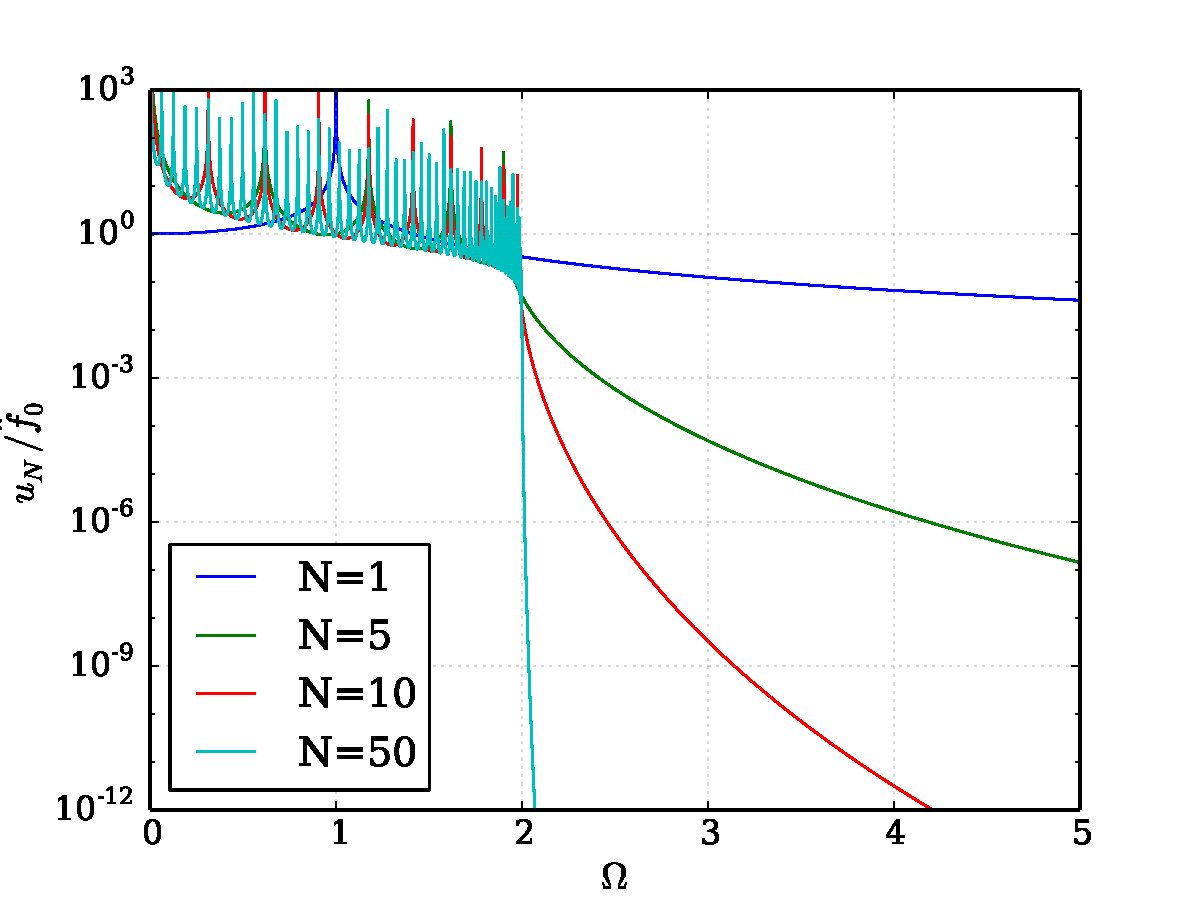
\includegraphics[height=8cm]{img/single_finite.pdf} 
\caption{Frequency response for a finite mass-spring lattice.}\label{fig:single-finite}
\end{figure}

We can see that for $N$ big enough there is not propagation for frequencies larger than $\Omega=2$, what was expected based on the Bloch analysis and the dispersion curves presented in Figure \ref{fig:spring-mass-dispersion}.


%% 
\section{Diatomic crystal}
\begin{figure}[h]
\centering
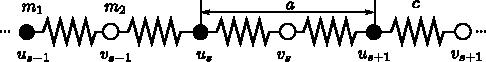
\includegraphics[height=1.5cm]{img/diatomic-crystal.pdf} 
\caption{Lattice made with spring and two species of masses.}
\end{figure}
We write the equations of motion under the assumption that each plane interacts only with its nearest-neighbour planes and that the force constants are identical between all pairs of nearest-neighbour planes.
\begin{subequations}
\begin{align}
m_1\frac{d^2 u_s}{dt^2} = c(v_s+v_{s-1}-2u_s); \\
m_2\frac{d^2 v_s}{dt^2} = c(u_{s+1}+u_{s}-2v_s).
\end{align}
\label{eq:diatomic-eq}
\end{subequations}
We look for a solution in the form of a traveling wave, now with different amplitudes $u$, $v$ on alternate phases:
\begin{subequations}
\begin{align}
u_s = u\exp(ika)\exp(-i\omega t); \\
v_s = v\exp(ika)\exp(-i\omega t).
\end{align}
\label{eq:diatomic-sol}
\end{subequations}
Replacing (\ref{eq:diatomic-sol}) in (\ref{eq:diatomic-eq}) we have
\begin{align*}
-\omega^2 m_1 u = cv[1+\exp(-ika)] - 2cu; \\
-\omega^2 m_2 v = cu[1+\exp(ika)] - 2cv.
\end{align*}
It has no trivial solution only if the determinant vanishes, i.e.
\[\begin{vmatrix}
2c - m_1 \omega^2 & -c[1+\exp(-ika)] \\ 
-c[1+\exp(ika)] & 2c - m_2 \omega^2
\end{vmatrix}   = 0,\]
or
\begin{equation}
m_1 m_2 \omega^4 - 2c(m_1 + m_2)\omega^2 + 2c^2(1-\cos ka)=0 \enspace .
\end{equation}
Solving this biquadratic equation and doing some algebraic manipulations, we get
\begin{equation}
\omega^2 = \frac{c}{m_1 m_2} \left[ m_1+m_2 \pm \sqrt{(m_1+m_2)^2-2m_1 m_2(1-\cos ka)}\right] \enspace .
\end{equation}
\begin{figure}[h]
\centering
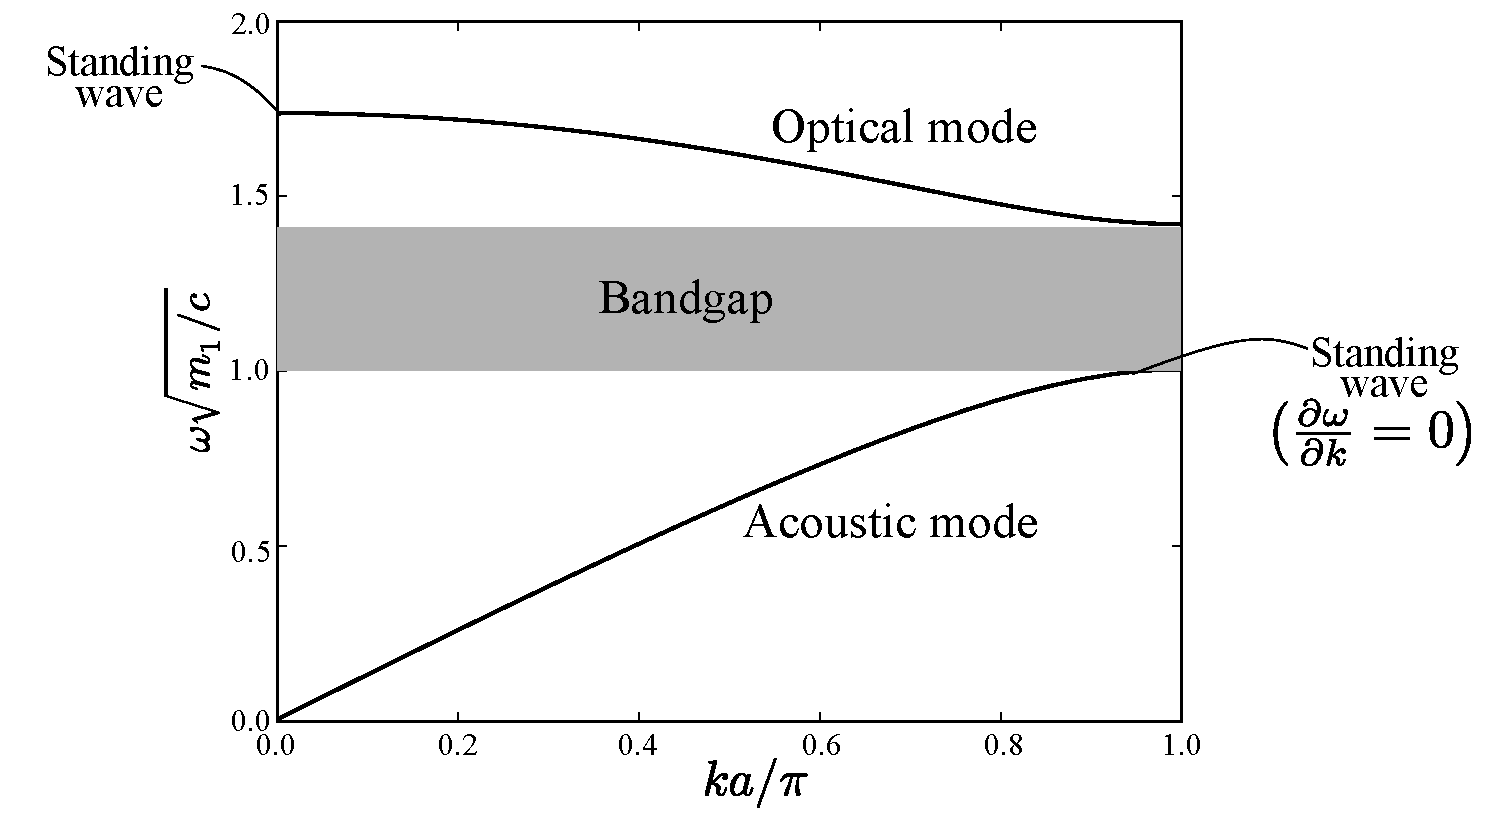
\includegraphics[height=8cm]{img/diatomic-plot.pdf} 
\caption{Optical and acoustical branches of the dispersion relation for a diatomic linear lattice. The values are computed for a ratio $m_2/m_1 = 2$.}
\label{fig:diatomic_dispersion}
\end{figure}
Let's examine the limiting cases $ka<<1$ and $ka=\pm \pi$ at the boundary zone. For small $ka$ we have $\cos ka \approx 1 - \frac{1}{2}k^2a^2 + \cdots$, and the two roots are
\begin{align}
\omega^2 &\approx 2c\left(\frac{1}{m_1} + \frac{1}{m_2}\right)\quad \mbox{(optical branch)}\\
\omega^2 &\approx \frac{\frac{1}{2}c}{m_1+m_2}k^2a^2\quad \mbox{(acoustical branch)} \enspace  .
\end{align}
At $k_{max}=\pm\pi/a$ the roots are
\[\omega^2 = 2c/m_1,\quad \omega^2 = 2c/m_2 \enspace .\]

\subsection{Finite case}
\begin{figure}[h]
\centering
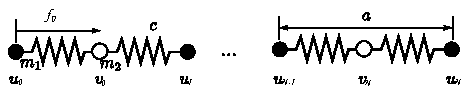
\includegraphics[width=4in]{img/diatomic-finite.pdf} 
\caption{Finite \emph{lattice} made with spring and two species of masses.}
\label{fig:diatomic-finite}
\end{figure}

For the case of a single unit cell the system of equation read
\begin{align*}
&-c(u_0 - v_0) + f_0 = -\omega^2 m_1 u_0\\
&-c(v_0 - u_0) - c(v_0 - u_1) = -\omega^2 m_2 v_0\\
&-c(u_1 - v_0) = -\omega^2 m_1 u_1 \enspace ,
\end{align*}
or
\[
c\begin{bmatrix}
-1 & 1 & 0 \\ 
1 & -2 & 1 \\ 
0 & 1 & -1
\end{bmatrix}
\begin{Bmatrix}
u_0 \\ 
v_0 \\ 
u_1
\end{Bmatrix} + m_1\omega^2\begin{bmatrix}
1 & 0 & 0 \\ 
0 & \frac{m_2}{m_1} & 0 \\ 
0 & 0 & 1
\end{bmatrix}
\begin{Bmatrix}
u_0 \\ 
v_0 \\ 
u_1
\end{Bmatrix} = 
\begin{Bmatrix}
-f_0 \\ 
0 \\ 
0
\end{Bmatrix}  \enspace ,
\]
making $\hat{f}_0=f_0/c$, $\Omega^2=\omega^2/\omega_0^2$, $\omega_0^2=c/m_1$, $\mu=m_2/m_1$ we obtain
\begin{equation}
\begin{bmatrix}
-1 + \Omega^2 & 1 & 0 \\ 
1 & -2 + \mu\Omega^2 & 1 \\ 
0 & 1 & -1 + \Omega^2
\end{bmatrix}
\begin{Bmatrix}
u_0 \\ 
v_0 \\ 
u_1
\end{Bmatrix}  = 
\begin{Bmatrix}
-\hat{f}_0 \\ 
0 \\ 
0
\end{Bmatrix} \enspace .
\label{eq:1_cell_diatomic}
\end{equation}

The solution of this system is given by
\begin{align*}
u_0 &= \frac{-\hat{f}_0 (\mu\Omega^4 - \mu\Omega^2 - 2\Omega^2 +1)}{\Omega^2 (\Omega - 1) (\Omega +1) (\mu\Omega^2 - \mu - 2)}\\
v_0 &= \frac{\hat{f}_0}{\Omega^2 (\mu\Omega^2 - \mu - 2)}\\
u_1 &= \frac{-\hat{f}_0}{\Omega^2 (\Omega - 1) (\Omega +1) (\mu\Omega^2 - \mu - 2)} \enspace ,
\end{align*}
thus, the response is given by
\begin{equation}
\frac{u_1}{\hat{f}_0} = \frac{-1}{\Omega^2 (\Omega - 1) (\Omega +1) (\mu\Omega^2 - \mu - 2)} \enspace .
\label{eq:1_cell_diatomic_response}
\end{equation}

For the case of two unit cells the system of (dimensionless) equations is written as
\begin{equation}
\begin{bmatrix}
-1 + \Omega^2 & 1 & 0 & 0 & 0 \\ 
1 & -2+ \mu\Omega^2 & 1 & 0 & 0 \\ 
0 & 1 & -2+ \Omega^2 & 1 & 0 \\ 
0 & 0 & 1 & -2+ \mu\Omega^2 & 1 \\ 
0 & 0 & 0 & 1 & -1+ \Omega^2
\end{bmatrix}
\begin{Bmatrix}
u_0 \\ 
v_0 \\ 
u_1 \\ 
v_1 \\ 
u_2
\end{Bmatrix}  =
\begin{Bmatrix}
-\hat{f}_0 \\ 
0 \\ 
0 \\ 
0 \\ 
0
\end{Bmatrix}  \enspace ,
\end{equation}
with solutions
\begin{align*}
u_0 &= \frac{-\hat{f}_0({\mu}^2\Omega^8 - 3{\mu}^2\Omega^6 - 4\mu\Omega^6 + 2{\mu}^2\Omega^4 + 9\mu\Omega^4 + 4\Omega^4 - 4\mu\Omega^2 - 6\Omega^2 + 1) }{\Omega^2(\mu\Omega^4 - 3\mu\Omega^2 - 2\Omega^2 + 2\mu + 3) (\mu\Omega^4 - \mu\Omega^2 - 2\Omega^2 + 1) }\\
v_0 &= \frac{\hat{f}_0(\mu\Omega^6 - 3\mu\Omega^4 - 2\Omega^4 + 2\mu\Omega^2 + 4\Omega^2 - 1) }{\Omega^2(\mu\Omega^4 - 3\mu\Omega^2 - 2\Omega^2 + 2\mu + 3) (\mu\Omega^4 - \mu\Omega^2 - 2\Omega^2 + 1) }\\
u_1 &= \frac{-\hat{f}_0}{\Omega^2(\mu\Omega^4 - 3\mu\Omega^2 - 2\Omega^2 + 2\mu + 3) }\\
v_1 &= \frac{\hat{f}_0(\Omega - 1) (\Omega + 1) }{\Omega^2(\mu\Omega^4 - 3\mu\Omega^2 - 2\Omega^2 + 2\mu + 3) (\mu\Omega^4 - \mu\Omega^2 - 2\Omega^2 + 1) }\\
u_2 &= \frac{-\hat{f}_0}{\Omega^2(\mu\Omega^4 - 3\mu\Omega^2 - 2\Omega^2 + 2\mu + 3) (\mu\Omega^4 - \mu\Omega^2 - 2\Omega^2 + 1)} \enspace ,
\end{align*}
then, the response is
\begin{equation}
\frac{u_2}{\hat{f}_0} = \frac{-1}{\Omega^2(\mu\Omega^4 - 3\mu\Omega^2 - 2\Omega^2 + 2\mu + 3) (\mu\Omega^4 - \mu\Omega^2 - 2\Omega^2 + 1)} \enspace .
\label{eq:2_cell_diatomic_response}
\end{equation}

For $N$ unit cells the (dimensionless) system of equation is of the form
\begin{equation}
\mathbb{A}
\begin{Bmatrix}
u_0 \\ 
v_0 \\ 
u_1 \\ 
\vdots \\ 
u_{N-1} \\ 
v_{N-1} \\ 
u_N
\end{Bmatrix} = 
\begin{Bmatrix}
-\hat{f}_0 \\ 
0 \\ 
0 \\ 
0 \\ 
0 \\ 
0 \\ 
0
\end{Bmatrix}
\end{equation}
with
\[\mathbb{A} = \begin{bmatrix}
-1 + \Omega^2 & 1 & 0 & \cdots & 0 & 0 & 0 \\ 
1 & -2 +\mu \Omega^2 & 1 & \cdots & 0 & 0 & 0 \\ 
0 & 1 & -2 + \Omega^2 & \cdots & 0 & 0 & 0 \\ 
\vdots & \vdots & \vdots & \ddots & \vdots & \vdots & \vdots \\ 
0 & 0 & 0 & \cdots & -2 + \Omega^2 & 1 & 0 \\ 
0 & 0 & 0 & \cdots & 1 & -2 +\mu \Omega^2 & 1 \\ 
0 & 0 & 0 & \cdots & 0 & 1 & -1 + \Omega^2
\end{bmatrix} \]


One more time, the matrix present a structure and it might be  possible that the system has a closed solution. Here, we solved the system numerically and plotted the ratio $u_N/\hat{f}_0$ for different $N$ values and a mass ratio $\mu=m_2/m_1=2$ (Figure \ref{fig:diatomic-finite}).
\begin{figure}[h]
\centering
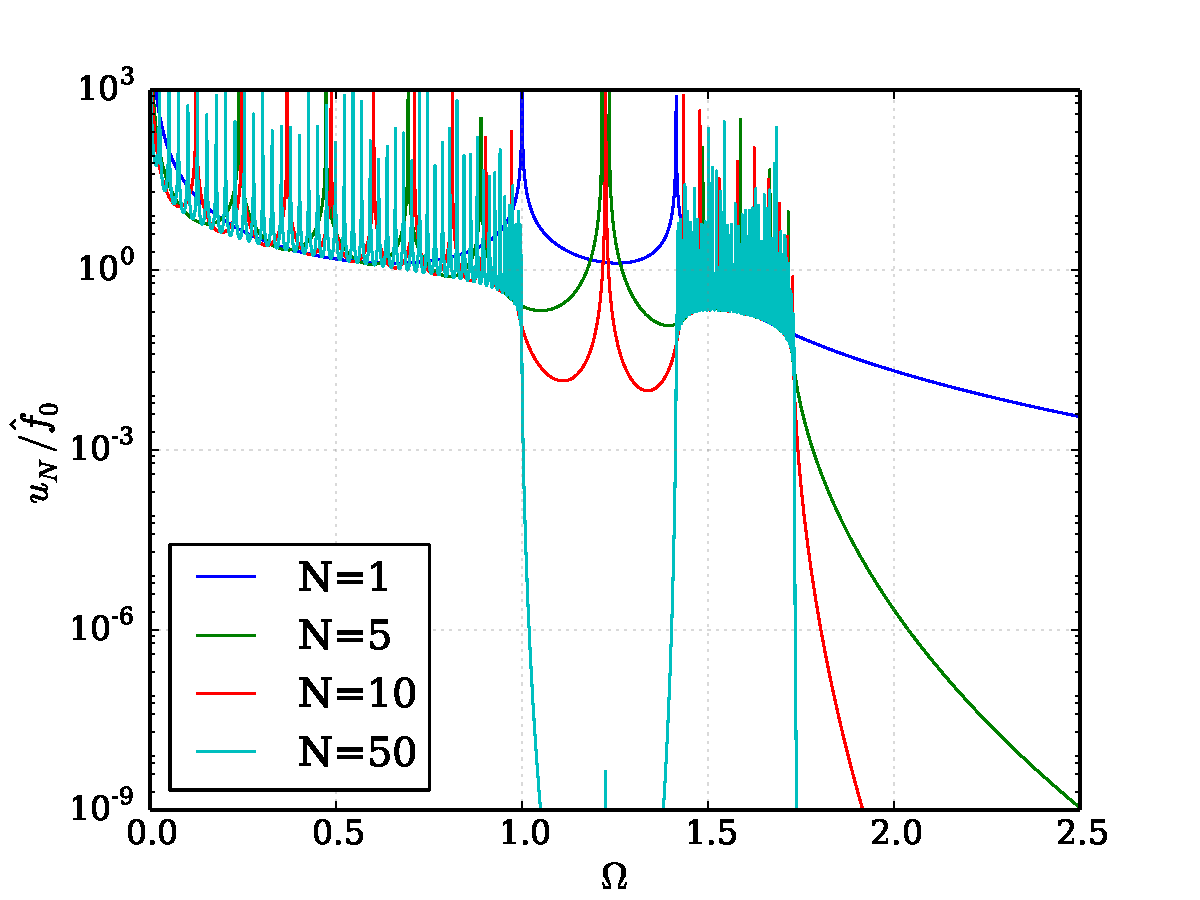
\includegraphics[height=8cm]{img/diatomic_finite.pdf} 
\caption{Frequency response for a finite mass-spring lattice for unit cell composed of two different masses.}
\label{fig:diatomic-finite-disp}
\end{figure}

We can see that for $N$ big enough there is not propagation for frequencies in the interval $\Omega \in [\sqrt{2/\mu}, \sqrt{2/\mu}]$, and for $\Omega > \sqrt{\frac{2}{\mu}(1 + \mu)}$, 
what was expected based on the Bloch analysis and the dispersion curves presented in Figure \ref{fig:diatomic_dispersion}. The mass ratio used was $\mu=2$, what gives as interval $\Omega \in [1, \sqrt{2}]$ and a cut frequency of $\Omega = \sqrt{3}$, that are clearly depicted in Figure \ref{fig:diatomic_dispersion}.


\section{Three masses lattice}
The equations are
\begin{subequations}
\begin{align}
m_1\frac{d^2 u_s}{dt^2} = c(v_s+w_{s-1}-2u_s); \\
m_2\frac{d^2 v_s}{dt^2} = c(w_{s}+u_{s}-2v_s);\\
m_3\frac{d^2 w_s}{dt^2} =c(u_{s+1}+v_{s}-2w_s).
\end{align}
\label{eq:three-masses}
\end{subequations}
After assumin an harmonic solution and apply Bloch conditions the following system is found
 \begin{equation}
\left[ \begin{matrix}
-2 & 1 & \exp(-ika) \\ 
1 & -2 & 1 \\ 
\exp(ika) & 1 & -2
\end{matrix}  \right] \left\lbrace \begin{matrix}
u \\ 
v \\ 
w
\end{matrix}  \right\rbrace = -\frac{\omega^2}{\omega_0^2}\left[ \begin{matrix}
1 & 0 & 0 \\ 
0 & \mu_1 & 0 \\ 
0 & 0 & \mu_2
\end{matrix} \right] \left\lbrace \begin{matrix}
u \\ 
v \\ 
w
\end{matrix} \right\rbrace \enspace , 
 \end{equation}
where $\omega_0^2=c/m_1$, $\mu_1 = m_2/m_1$ and $\mu_2=m_3/m_1$. The characteristic polynomial for this system is
\begin{equation}
\mu_1 \mu_2 x^3 - 2[\mu_1\mu_2 -\mu_1 -\mu_2]x^2 + 3[\mu_1+\mu_2+1]x+2[\cos ka -1] = 0 \enspace .
\end{equation}
Figure \ref{fig:three-masses} presents some dispersion curves for different mass ratios.
\begin{figure}[h]
        \centering
        \begin{subfigure}[b]{0.49\textwidth}
                \includegraphics[width=\textwidth]{img/{spring_masses-3-m1=0.5-m2=3}.pdf}
                \caption{$\mu_1=1/2$, $\mu_2=3$.}
        \end{subfigure}\,
%
        \begin{subfigure}[b]{0.49\textwidth}
                \includegraphics[width=\textwidth]{img/{spring_masses-3-m1=0.5-m2=10}.pdf}
                \caption{$\mu_1=1/2$, $\mu_2=10$.}
        \end{subfigure}\\
%
        \begin{subfigure}[b]{0.49\textwidth}
                \includegraphics[width=\textwidth]{img/{spring_masses-3-m1=2-m2=3}.pdf}
                \caption{$\mu_1=2$, $\mu_2=3$.}
        \end{subfigure}\,
%
        \begin{subfigure}[b]{0.49\textwidth}
                \includegraphics[width=\textwidth]{img/{spring_masses-3-m1=2-m2=10}.pdf}
                \caption{$\mu_1=2$, $\mu_2=10$.}
        \end{subfigure}
        \caption{Dispersion curves for different values of mass ratios $\mu_1, \mu_2$.}\label{fig:three-masses}
\end{figure}

\subsection{Finite case}
We can repeat the analysis done for one-mass and two-masses unit cells for the case of three-masses unit cell. In this case, the closed solution for one and two unit cells is not shown since the expression are large compared with the other two cases. Nevertheless, we present the equation form for the $N$ cells case
\begin{equation}
  \mathbb{A}\begin{Bmatrix}
  u_0 \\ 
  v_0 \\ 
  w_0 \\ 
  u_1 \\ 
  \vdots \\ 
  u_{N-1} \\ 
  v_{N-1} \\ 
  w_{N-1} \\ 
  u_N
  \end{Bmatrix} = 
  \begin{Bmatrix}
  -\hat{f}_0 \\ 
  0 \\ 
  0 \\ 
  0 \\ 
  \vdots \\ 
  0 \\ 
  0 \\ 
  0 \\ 
  0
\end{Bmatrix} \enspace ,
\end{equation}
with
\[\mathbb{A} = \begin{bmatrix}
 -1 + \Omega^2 & 1 & 0 & 0 & 0 & 0 & 0 & 0 & 0 \\ 
 1 & -2 + \mu_1\Omega^2 & 1 & 0 & \cdots & 0 & 0 & 0 & 0 \\ 
 0 & 1 & -2 + \mu_2\Omega^2 & 1 & \cdots & 0 & 0 & 0 & 0 \\ 
 0 & 0 & 1 & -2 + \Omega^2 & \cdots & 0 & 0 & 0 & 0 \\ 
 \vdots & \vdots & \vdots & \vdots & \ddots & \vdots & \vdots & \vdots & \vdots \\ 
 0 & 0 & 0 & 0 & \cdots & -2 + \Omega^2 & 1 & 0 & 0 \\ 
 0 & 0 & 0 & 0 & \cdots & 1 & -2 + \mu_1\Omega^2 & 0 & 0 \\ 
 0 & 0 & 0 & 0 & \cdots & 0 & 1 & -2 + \mu_2\Omega^2 & 1 \\ 
 0 & 0 & 0 & 0 & \cdots & 0 & 0 & 1 & -1 + \Omega^2
 \end{bmatrix}\]
 
Figure \ref{fig:three-finite} presents the frequency response for this case (computed numerically) for different mass ratios $\mu_1$ and $\mu_2$.
\begin{figure}[h]
        \centering
        \begin{subfigure}[b]{0.49\textwidth}
                \includegraphics[width=3in]{img/{three_finite-m1=0.5-m2=3}.pdf}
                \caption{$\mu_1=1/2$, $\mu_2=3$.}
        \end{subfigure}\,
%
        \begin{subfigure}[b]{0.49\textwidth}
                \includegraphics[width=3in]{img/{three_finite-m1=0.5-m2=10}.pdf}
                \caption{$\mu_1=1/2$, $\mu_2=10$.}
        \end{subfigure}\\
%
        \begin{subfigure}[b]{0.49\textwidth}
                \includegraphics[width=3in]{img/{three_finite-m1=2-m2=3}.pdf}
                \caption{$\mu_1=2$, $\mu_2=3$.}
        \end{subfigure}\,
%
        \begin{subfigure}[b]{0.49\textwidth}
                \includegraphics[width=3in]{img/{three_finite-m1=2-m2=10}.pdf}
                \caption{$\mu_1=2$, $\mu_2=10$.}
        \end{subfigure}
        \caption{Frequency response for a finite mass-spring lattice for unit cell composed of three different masses for different mass ratios.}\label{fig:three-finite}
\end{figure}

The bandgap regions and cut frequencies are (essentially) the same as those presented in the dispersion relations, Figure \ref{fig:three-masses}.

\section{2D square lattice}
For the simple cases shown before is easy to formulate the complete balance of forces taking into account the first neighbours. In general is easier to take the unit cell for the lattice and find the resulting system through row and column operations, just as exemplified before. 
\begin{figure}[h]
\centering
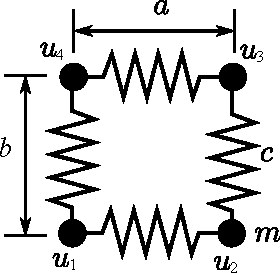
\includegraphics[height=5cm]{img/spring-square.pdf} 
\caption{Unit cell for a two dimensional square lattice with a unique species.}
\end{figure}
The system of equation in frequency domain is
\begin{equation}
c\begin{bmatrix}
-1 & 0 & 1 & 0 & 0 & 0 & 0 & 0 \\ 
0 & -1 & 0 & 0 & 0 & 0 & 0 & 1 \\ 
1 & 0 & -1 & 0 & 0 & 0 & 0 & 0 \\ 
0 & 0 & 0 & -1 & 0 & 1 & 0 & 0 \\ 
0 & 0 & 0 & 0 & -1 & 0 & 1 & 0 \\ 
0 & 0 & 0 & 1 & 0 & -1 & 0 & 0 \\ 
0 & 0 & 0 & 0 & 1 & 0 & -1 & 0 \\ 
0 & 1 & 0 & 0 & 0 & 0 & 0 & -1
\end{bmatrix} \begin{Bmatrix}
u_1 \\ 
v_1 \\ 
u_2 \\ 
v_2 \\ 
u_3 \\ 
v_3 \\ 
u_4 \\ 
v_4
\end{Bmatrix}= -\frac{\omega}{4}m \mathbb{I}_8
\begin{Bmatrix}
u_1 \\ 
v_1 \\ 
u_2 \\ 
v_2 \\ 
u_3 \\ 
v_3 \\ 
u_4 \\ 
v_4
\end{Bmatrix} \enspace ,
\end{equation}
and after applying the row operations for the Bloch-conditions imposition, we get
\begin{equation}
\frac{4c}{m}\begin{bmatrix}
1 - \cos(k_x a) & 0 \\ 
0 & 1-\cos(k_y b)
\end{bmatrix} \begin{Bmatrix}
u_1 \\ 
v_1 
\end{Bmatrix} = \omega^2 \begin{Bmatrix}
u_1 \\ 
v_1 
\end{Bmatrix} .
\end{equation}
Or, equivalently
\begin{equation}
\omega_x^2 = \frac{8c}{m}\left( \sin \frac{1}{2}k_x a\right)^2,\qquad \omega_y^2 = \frac{8c}{m}\left( \sin \frac{1}{2}k_y b \right)^2 \enspace .
\end{equation}
Figure \ref{fig:square-disp} shows the dispersion relation for this problem.
\begin{figure}[h]
\centering
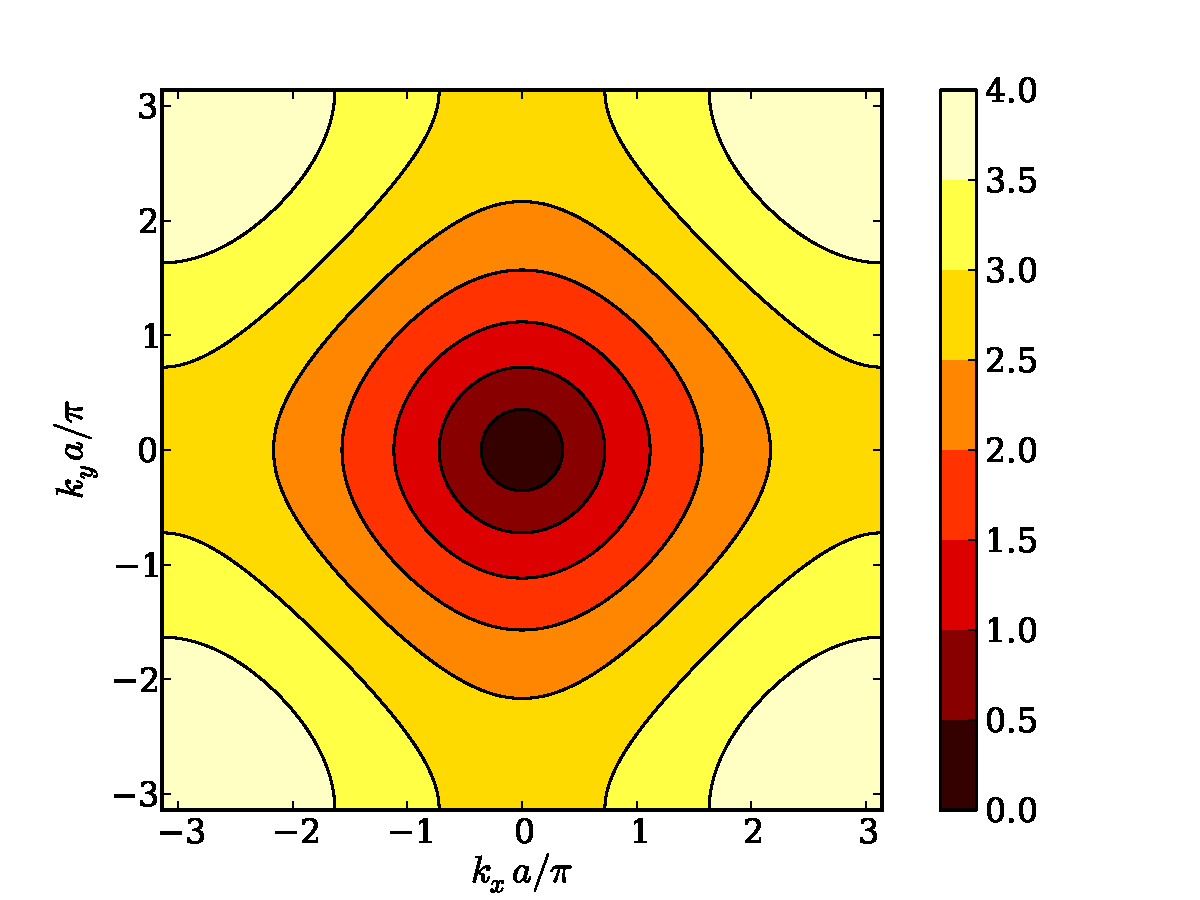
\includegraphics[width=4in]{img/square-disp.pdf} 
\caption{Dispersion relations--shown as isofrequency contours.}\label{fig:square-disp}
\end{figure}

It is customary to plot the dispersion relations over the irreducible Brillouin zone, this is depicted in Figure \ref{fig:square-disp-irreducible} for the square lattice.
\begin{figure}[h]
\centering
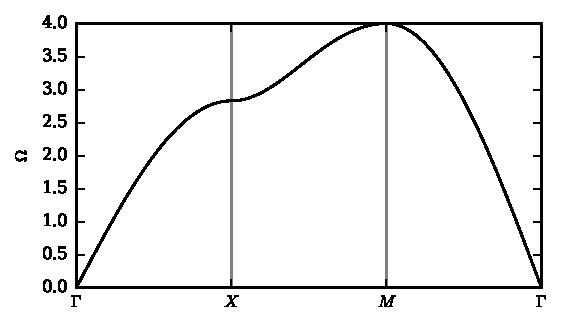
\includegraphics[width=4in]{img/square-disp-irreducible.pdf} 
\caption{Dispersion relations over the irreducible Brillouin zone}
\label{fig:square-disp-irreducible}
\end{figure}




\section{2D rectangular lattice with diagonal springs}
In this case we have a rectangular cell with springs with constant $c$ in the sides. We added diagonal springs with constants $c_d$ (see Figure \ref{fig:square-diag}). It should be noted that the value $c_d$ is the \emph{effective} spring in the $x$ and $y$ directions --they are the same for a square lattice, in the case of $a\neq b$ the constants should vary.
\begin{figure}[h]
\centering
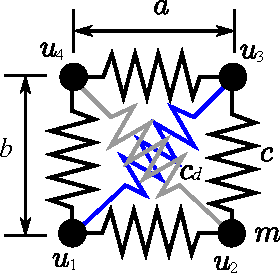
\includegraphics[height=5cm]{img/spring-square-diag.pdf} 
\caption{Unit cell for a two dimensional square lattice with a unique species and diagonal springs.}\label{fig:square-diag}
\end{figure}

The system of equation in frequency domain is
\begin{equation}
\mathbb{K}
\begin{Bmatrix}
u_1 \\ 
v_1 \\ 
u_2 \\ 
v_2 \\ 
u_3 \\ 
v_3 \\ 
u_4 \\ 
v_4
\end{Bmatrix} = -\frac{\omega^2}{4}m \mathbb{I}_8
\begin{Bmatrix}
u_1 \\ 
v_1 \\ 
u_2 \\ 
v_2 \\ 
u_3 \\ 
v_3 \\ 
u_4 \\ 
v_4
\end{Bmatrix}
\end{equation}
with
\[\mathbb{K} = \begin{bmatrix}
-c_{d}-c_{1} & 0 & c_{1} & 0 & c_{d} & 0 & 0 & 0\cr
0 & -c_{d}-c_{2} & 0 & 0 & 0 & c_{d} & 0 & c_{2}\cr
c_{1} & 0 & -c_{d}-c_{1} & 0 & 0 & 0 & c_{d} & 0\cr
0 & 0 & 0 & -c_{d}-c_{2} & 0 & c_{2} & 0 & c_{d}\cr
c_{d} & 0 & 0 & 0 & -c_{d}-c_{1} & 0 & c_{1} & 0\cr
0 & c_{d} & 0 & c_{2} & 0 & -c_{d}-c_{2} & 0 & 0\cr
0 & 0 & c_{d} & 0 & c_{1} & 0 & -c_{d}-c_{1} & 0\cr
0 & c_{2} & 0 & c_{d} & 0 & 0 & 0 & -c_{d}-c_{2}\end{bmatrix} \]

And the solutions are
\begin{align*}
\omega_1^2 &= \frac{4c_1}{m}\left[1 - \cos k_x a \right] + \frac{4 c_d}{m}\left[1 - \cos k_x a \cos k_y b \right]\\
\omega_2^2 &= \frac{4c_2}{m}\left[1 - \cos k_y a \right] + \frac{4 c_d}{m}\left[1 - \cos k_x a \cos k_y b \right] \enspace .
\end{align*}
equivalently (after some manipulations)
\begin{align}
\omega_1^2 &= \frac{8c_1}{m} \sin^2 \left(\frac{1}{2}k_x a\right)  + \frac{4c_d}{m} \left[\sin^2 \frac{1}{2}\left(k_x a + k_y b\right) + \sin^2 \frac{1}{2}\left(k_x a - k_y b\right)\right] \\
\omega_2^2 &= \frac{8c_2}{m} \sin^2 \left(\frac{1}{2}k_y b\right)  + \frac{4c_d}{m} \left[\sin^2 \frac{1}{2}\left(k_x a + k_y b\right) + \sin^2 \frac{1}{2}\left(k_x a - k_y b\right)\right]  
\end{align}
We recover the square lattice (without diagonals) making $c_d=0$. The dispersion curves for this problem varying the ratio $c_d/c$ are shown in Figure \ref{fig:square-diag-disp}.
\begin{figure}[h]
        \centering
        \begin{subfigure}[b]{0.49\textwidth}
                \includegraphics[width=\textwidth]{img/{square-diag-cd=0.1}.pdf}
                \caption{$c_d/c = 0.1$ and $a=b$.}
        \end{subfigure}\,
%
        \begin{subfigure}[b]{0.49\textwidth}
                \includegraphics[width=\textwidth]{img/{square-diag-cd=0.707107}.pdf}
                \caption{$c_d/c = \sqrt{2}/2$ and $a=b$.}
        \end{subfigure}\\
%
        \begin{subfigure}[b]{0.49\textwidth}
                \includegraphics[width=\textwidth]{img/{square-diag-cd=1}.pdf}
                \caption{$c_d/c = 1$ and $a=b$.}
        \end{subfigure}\,
%
        \begin{subfigure}[b]{0.49\textwidth}
                \includegraphics[width=\textwidth]{img/{square-diag-cd=10}.pdf}
                \caption{$c_d/c = 10$ and $a=b$.}
        \end{subfigure}
        \caption{Dispersion curves for different values of spring ratios $c_d/c$.}\label{fig:square-diag-disp}
\end{figure}



\begin{figure}[h]
        \centering
        \begin{subfigure}[b]{0.49\textwidth}
                \includegraphics[width=\textwidth]{img/{square-diag-irreducible-cd=0.1}.pdf}
                \caption{$c_d/c = 0.1$ and $a=b$.}
        \end{subfigure}\,
%
        \begin{subfigure}[b]{0.49\textwidth}
                \includegraphics[width=\textwidth]{img/{square-diag-irreducible-cd=0.707107}.pdf}
                \caption{$c_d/c = \sqrt{2}/2$ and $a=b$.}
        \end{subfigure}\\
%
        \begin{subfigure}[b]{0.49\textwidth}
                \includegraphics[width=\textwidth]{img/{square-diag-irreducible-cd=1}.pdf}
                \caption{$c_d/c = 1$ and $a=b$.}
        \end{subfigure}\,
%
        \begin{subfigure}[b]{0.49\textwidth}
                \includegraphics[width=\textwidth]{img/{square-diag-irreducible-cd=10}.pdf}
                \caption{$c_d/c = 10$ and $a=b$.}
        \end{subfigure}
        \caption{Dispersion curves for different values of spring ratios $c_d/c$.}
        \label{fig:square-diag-disp-irreducible}
\end{figure}

\section{2D square lattice with body mass and diagonal springs}
In this case we have a rectangular cell with springs with constant $c$ in the sides. We added a second mass $m_2$ to the center of the cell, and diagonal springs with constant $c_d$ (see Figure \ref{fig:square-bcc}). It should be noted that the value $c_d$ is the \emph{effective} spring in the $x$ and $y$ directions --they are the same for a square lattice, in the case of $a\neq b$ the constants should vary.
\begin{figure}[h]
\centering
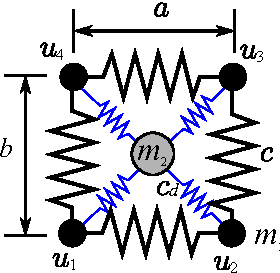
\includegraphics[height=5cm]{img/spring-square-bcc.pdf} 
\caption{Unit cell for a two dimensional square lattice with a unique species in the corners and another one in the center that is linked by diagonal springs.}\label{fig:square-bcc}
\end{figure}
\begin{equation}
\mathbb{K}
\begin{Bmatrix}
u_1 \\ 
v_1 \\ 
u_2 \\ 
v_2 \\ 
u_3 \\ 
v_3 \\ 
u_4 \\ 
v_4 \\
u_5 \\
v_5
\end{Bmatrix}  = -\omega^2 \mathbb{M}
\begin{Bmatrix}
u_1 \\ 
v_1 \\ 
u_2 \\ 
v_2 \\ 
u_3 \\ 
v_3 \\ 
u_4 \\ 
v_4 \\
u_5 \\
v_5
\end{Bmatrix} 
\end{equation}
with
\[\mathbb{K} =\begin{bmatrix}
-{c}_{s}-{c}_{d} & 0 & {c}_{s} & 0 & 0 & 0 & 0 & 0 & {c}_{d} & 0\cr
 0 & -{c}_{s}-{c}_{d} & 0 & 0 & 0 & 0 & 0 & {c}_{s} & 0 & {c}_{d}\cr
 {c}_{s} & 0 & -{c}_{s}-{c}_{d} & 0 & 0 & 0 & 0 & 0 & {c}_{d} & 0\cr
 0 & 0 & 0 & -{c}_{s}-{c}_{d} & 0 & {c}_{s} & 0 & 0 & 0 & {c}_{d}\cr
 0 & 0 & 0 & 0 & -{c}_{s}-{c}_{d} & 0 & {c}_{s} & 0 & {c}_{d} & 0\cr
 0 & 0 & 0 & {c}_{s} & 0 & -{c}_{s}-{c}_{d} & 0 & 0 & 0 & {c}_{d}\cr
 0 & 0 & 0 & 0 & {c}_{s} & 0 & -{c}_{s}-{c}_{d} & 0 & {c}_{d} & 0\cr
 0 & {c}_{s} & 0 & 0 & 0 & 0 & 0 & -{c}_{s}-{c}_{d} & 0 & {c}_{d}\cr
 {c}_{d} & 0 & {c}_{d} & 0 & {c}_{d} & 0 & {c}_{d} & 0 & -4\,{c}_{d} & 0\cr
 0 & {c}_{d} & 0 & {c}_{d} & 0 & {c}_{d} & 0 & {c}_{d} & 0 & -4\,{c}_{d}\end{bmatrix},\]
and
\[\mathbb{M} = \begin{bmatrix}
\frac{m_1}{4}\mathbb{I}_6 & 0 \\ 
0 & m_2\mathbb{I}_2
\end{bmatrix} \enspace . \]

After applying the Bloch theorem we obtain (showing just the lower diagonal due to the Hermiticity)
\[\mathbb{K}_R = \begin{bmatrix}
-4\left[c_d - c_s(\cos(k_y a) - 1)\right]  & \bullet & \bullet & \bullet\\
 0 & -4\left[c_d - c_s(\cos(k_y b) - 1)\right]  & \bullet & \bullet\\
 c_d\left( e^{i\, k_x a}+1\right) \left( e^{i\, k_y b}+1\right)  & 0 & -4c_d & \bullet\\
 0 & c_d\left( e^{i\, k_x a}+1\right) \left( e^{i\, k_y b}+1\right)  & 0 & -4c_d
\end{bmatrix}\]
and
\[\mathbb{M}_R =\begin{bmatrix}
m_1\mathbb{I}_2 & 0 \\ 
0 & m_2\mathbb{I}_2
\end{bmatrix} \enspace .\]

The eigenvalues for this problem are lengthy, but a second order expansion around $(k_x,k_y)=(0,0)$ (linear in the case o its square root) is shown
\begin{align*}
\omega_1^2 =& \frac{2c_s (k_x a)^2 + c_d\left((k_x a)^2 + (k_y b)^2\right)}{m_1 + m_2}\\
\omega_2^2 =& \frac{2c_s (k_y b)^2 + c_d\left((k_x a)^2 + (k_y b)^2\right)}{m_1 + m_2}\\
\omega_3^2 =& \frac{2c_s (k_x a)^2 + 2c_d\left[2m_1^2 + 2m_2^2 + \left(4 - (k_x a)^2 +(k_y b)^2\right)m_1 m_2\right] } {m_1 m_2 (m_2 + m_1)}\\
\omega_4^2 =& \frac{2c_s (k_y b)^2 + 2c_d\left[2m_1^2 + 2m_2^2 + \left(4 - (k_x a)^2 +(k_y b)^2\right)m_1 m_2\right] } {m_1 m_2 (m_2 + m_1)} \enspace .
\end{align*}
Assuming $a=b$, we can group the modes as degenerate ones and consider the most general propagation in the plane (due to the orthogonality)
\[\omega_{\text{low}}^2 = \frac{2 (c_s + c_d) (k_x^2 + k_y^2)a^2}{m_1 + m_2} \equiv \frac{2 (c_s + c_d) \mathbf{k}^2 a^2}{m_1 + m_2} \enspace ,\]
the same argument holds for the other two, giving
\[\omega_{\text{high}}^2 = \frac{2c_s \mathbf{k}^2a^2 + 2c_d\left[4m_1^2 + 4m_2^2 + \left(8 - \mathbf{k}^2 a^2\right)m_1 m_2\right] } {m_1 m_2 (m_2 + m_1)} \enspace .\]

Figure \ref{fig:square-bcc-disp} shows the dispersion modes for ratios $m_2/m_1=1$ and $c_d/c_s=1$.
\begin{figure}[h]
        \centering
        \begin{subfigure}[b]{0.49\textwidth}
                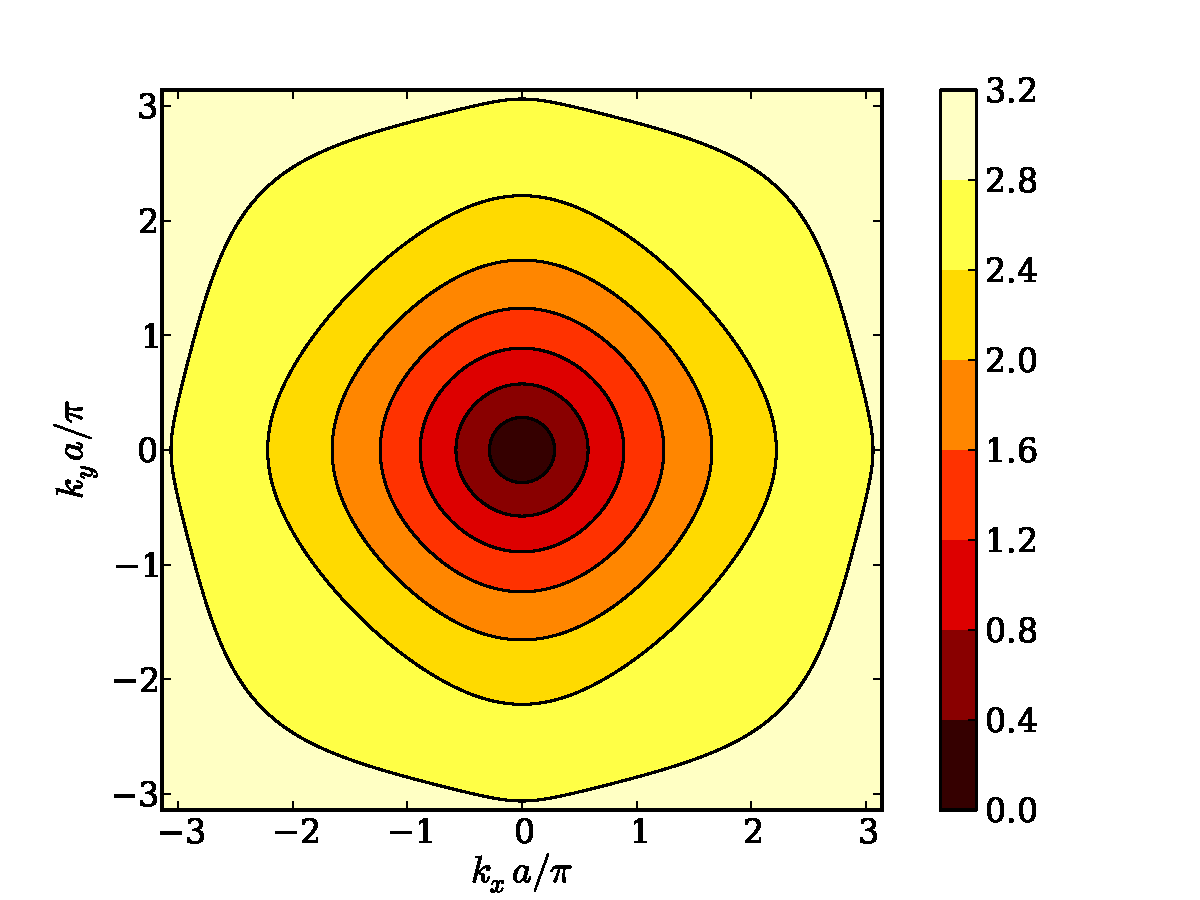
\includegraphics[width=\textwidth]{img/square-bcc-disp1-c=1-m=1.pdf}\caption{First branch.}
        \end{subfigure}\,
%
        \begin{subfigure}[b]{0.49\textwidth}
                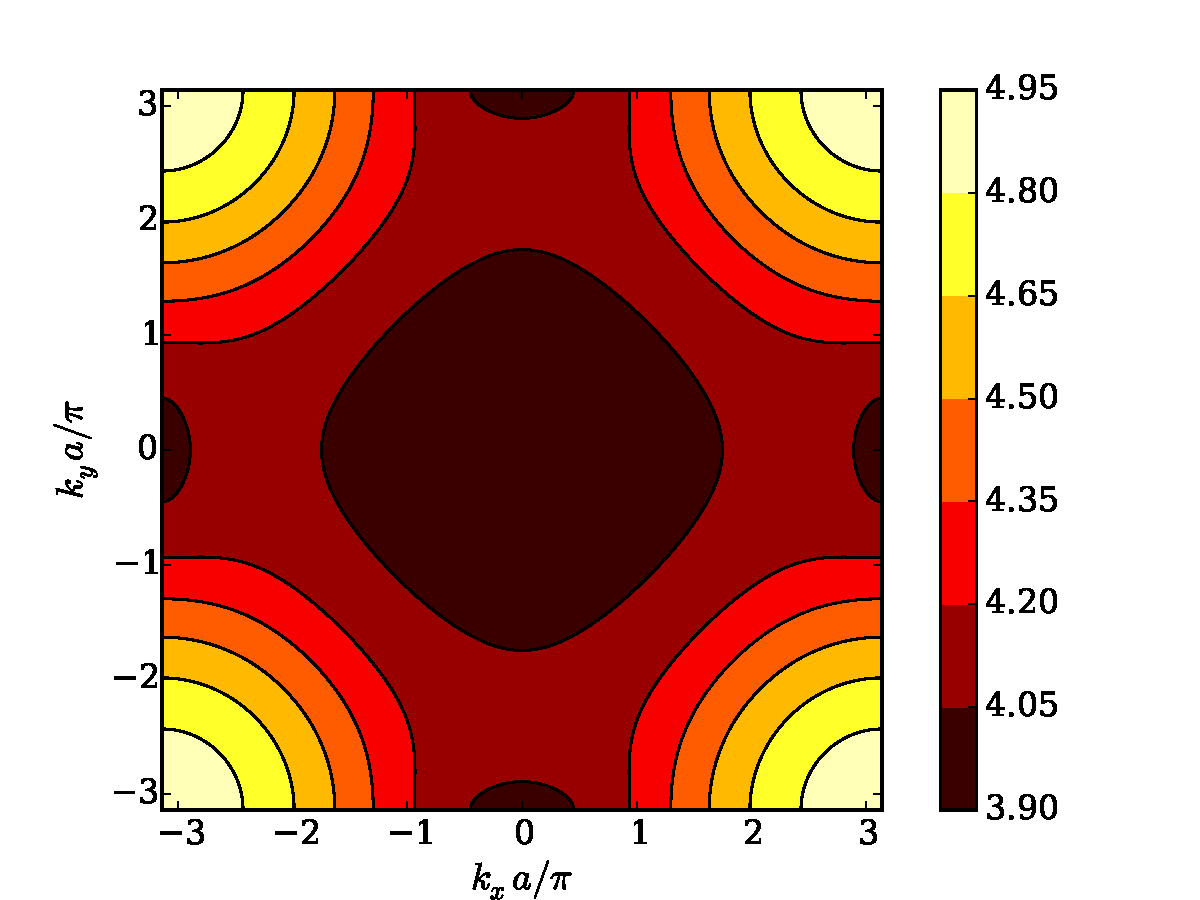
\includegraphics[width=\textwidth]{img/square-bcc-disp2-c=1-m=1.pdf}\caption{Second branch.}
         \end{subfigure}
 \caption{$c_d/c = 1$, $m_1/m_2=1$ and $a=b$.}\label{fig:square-bcc-disp}
\end{figure}
Figure \ref{fig:square-bcc-disp1} shows the first branch of the dispersion curves for different ratios $m_2/m_1$ and $c_d/c_s$.
\begin{figure}[h]
        \centering
        \begin{subfigure}[b]{0.49\textwidth}
                \includegraphics[width=\textwidth]{img/{square-bcc-disp1-c=0.1-m=1}.pdf}
                \caption{$c_d/c = 0.1$, $m_2/m_1=1$ and $a=b$.}
        \end{subfigure}\,
%
        \begin{subfigure}[b]{0.49\textwidth}
                \includegraphics[width=\textwidth]{img/{square-bcc-disp1-c=10-m=1}.pdf}
                \caption{$c_d/c = 10$, $m_2/m_1=1$ and $a=b$.}
        \end{subfigure}\\
%
        \begin{subfigure}[b]{0.49\textwidth}
                \includegraphics[width=\textwidth]{img/{square-bcc-disp1-c=1-m=0.1}.pdf}
                \caption{$c_d/c = 1$, $m_2/m_1=0.1$ and $a=b$.}
        \end{subfigure}\,
%
        \begin{subfigure}[b]{0.49\textwidth}
                \includegraphics[width=\textwidth]{img/{square-bcc-disp1-c=1-m=10}.pdf}
                \caption{$c_d/c = 1$, $m_2/m_1=10$ and $a=b$.}
        \end{subfigure}
        \caption{First branch of the dispersion curves.}\label{fig:square-bcc-disp1}
\end{figure}

Figure \ref{fig:square-bcc-disp2} shows the second branch of the dispersion curves for different ratios $m_2/m_1$ and $c_d/c_s$.
\begin{figure}[h]
        \centering
        \begin{subfigure}[b]{0.49\textwidth}
                \includegraphics[width=\textwidth]{img/{square-bcc-disp2-c=0.1-m=1}.pdf}
                \caption{$c_d/c = 0.1$, $m_2/m_1=1$ and $a=b$.}
        \end{subfigure}\,
%
        \begin{subfigure}[b]{0.49\textwidth}
                \includegraphics[width=\textwidth]{img/{square-bcc-disp2-c=10-m=1}.pdf}
                \caption{$c_d/c = 10$, $m_2/m_1=1$ and $a=b$.}
        \end{subfigure}\\
%
        \begin{subfigure}[b]{0.49\textwidth}
                \includegraphics[width=\textwidth]{img/{square-bcc-disp2-c=1-m=0.1}.pdf}
                \caption{$c_d/c = 1$, $m_2/m_1=0.1$ and $a=b$.}
        \end{subfigure}\,
%
        \begin{subfigure}[b]{0.49\textwidth}
                \includegraphics[width=\textwidth]{img/{square-bcc-disp2-c=1-m=10}.pdf}
                \caption{$c_d/c = 1$, $m_2/m_1=10$ and $a=b$.}
        \end{subfigure}
        \caption{Second branch of the dispersion curves.}\label{fig:square-bcc-disp2}
\end{figure}


\begin{figure}[h]
        \centering
        \begin{subfigure}[b]{0.49\textwidth}
                \includegraphics[width=3in]{img/{square-bcc-irreducible-c=0.1-m=1}.pdf}
                \caption{$c_d/c = 0.1$, $m_2/m_1=1$ and $a=b$.}
        \end{subfigure}\,
%
        \begin{subfigure}[b]{0.49\textwidth}
                \includegraphics[width=3in]{img/{square-bcc-irreducible-c=10-m=1}.pdf}
                \caption{$c_d/c = 10$, $m_2/m_1=1$ and $a=b$.}
        \end{subfigure}\\
%
        \begin{subfigure}[b]{0.49\textwidth}
                \includegraphics[width=3in]{img/{square-bcc-irreducible-c=1-m=0.1}.pdf}
                \caption{$c_d/c = 1$, $m_2/m_1=0.1$ and $a=b$.}
        \end{subfigure}\,
%
        \begin{subfigure}[b]{0.49\textwidth}
                \includegraphics[width=3in]{img/{square-bcc-irreducible-c=1-m=10}.pdf}
                \caption{$c_d/c = 1$, $m_2/m_1=10$ and $a=b$.}
        \end{subfigure}
        \caption{Dispersion curves over the irreducible Brillouin zone.}\label{fig:square-bcc-disp-irreducible}
\end{figure}


\section{Hexagonal Lattice}
In this case we have an hexagonal cell with springs with constant $c$ in the sides (see Figure \ref{fig:hexagon}). 
\begin{figure}[h]
\centering
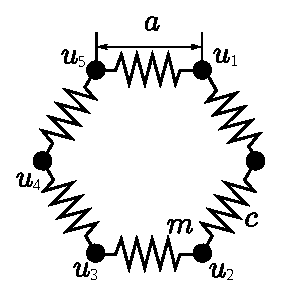
\includegraphics[height=5cm]{img/spring-hexagon.pdf} 
\caption{Unit cell for a two dimensional hexagonal lattice with a unique species in the corners.}\label{fig:hexagon}
\end{figure}
The system of equations to solve is one more time
\begin{equation}
\mathbb{K}
\begin{Bmatrix}
u_1 \\ 
v_1 \\ 
u_2 \\ 
v_2 \\ 
u_3 \\ 
v_3 \\ 
u_4 \\ 
v_4 \\
u_5 \\
v_5 \\
u_6 \\
v_6
\end{Bmatrix}  = -\omega^2 \mathbb{M}
\begin{Bmatrix}
u_1 \\ 
v_1 \\ 
u_2 \\ 
v_2 \\ 
u_3 \\ 
v_3 \\ 
u_4 \\ 
v_4 \\
u_5 \\
v_5 \\
u_6 \\
v_6
\end{Bmatrix} 
\end{equation}
with 
\setcounter{MaxMatrixCols}{12}
\[\mathbb{K} = \frac{c}{2}\begin{bmatrix}-3 & 0 & 1 & 0 & 0 & 0 & 0 & 0 & 0 & 0 & 2 & 0\cr
0 & -\sqrt{3} & 0 & \sqrt{3} & 0 & 0 & 0 & 0 & 0 & 0 & 0 & 0\cr
1 & 0 & -2 & 0 & 1 & 0 & 0 & 0 & 0 & 0 & 0 & 0\cr
0 & \sqrt{3} & 0 & -2\,\sqrt{3} & 0 & \sqrt{3} & 0 & 0 & 0 & 0 & 0 & 0\cr
0 & 0 & 1 & 0 & -3 & 0 & 2 & 0 & 0 & 0 & 0 & 0\cr
0 & 0 & 0 & \sqrt{3} & 0 & -\sqrt{3} & 0 & 0 & 0 & 0 & 0 & 0\cr
0 & 0 & 0 & 0 & 2 & 0 & -3 & 0 & 1 & 0 & 0 & 0\cr
0 & 0 & 0 & 0 & 0 & 0 & 0 & -\sqrt{3} & 0 & \sqrt{3} & 0 & 0\cr
0 & 0 & 0 & 0 & 0 & 0 & 1 & 0 & -2 & 0 & 1 & 0\cr
0 & 0 & 0 & 0 & 0 & 0 & 0 & \sqrt{3} & 0 & -2\,\sqrt{3} & 0 & \sqrt{3}\cr
2 & 0 & 0 & 0 & 0 & 0 & 0 & 0 & 1 & 0 & -3 & 0\cr
0 & 0 & 0 & 0 & 0 & 0 & 0 & 0 & 0 & \sqrt{3} & 0 & -\sqrt{3}
\end{bmatrix}\]
and
\[\mathbb{M} = \frac{m}{3}\mathbb{I}_{12} \enspace .  \]

After applying the Bloch theorem we obtain (showing just the lower diagonal due to the Hermiticity)
\[\mathbb{K}_R = c\begin{bmatrix}
-4 & \bullet & \bullet  & \bullet\cr
0 & -2\sqrt{3} & \bullet & \bullet\cr
e^{\frac{\sqrt{3}\,i k_y a}{2}-\frac{i k_x a}{2}}+e^{-\frac{\sqrt{3}\,i k_y a}{2}-\frac{i k_x a}{2}}+2\,e^{i k_x a}  & 0 & -4 & \bullet\cr
0 & e^{\frac{\sqrt{3}ik_y a}{2}-\frac{ik_x a}{2}}+e^{-\frac{\sqrt{3}ik_y a}{2}-\frac{ik_x a}{2}} & 0 & -2\sqrt{3}
\end{bmatrix}\]
and
\[\mathbb{M}_R = m \mathbb{I}_4 .\]

The eigenvalues for this problem are lengthy, but a second order expansion around $(k_x,k_y)=(0,0)$ (linear in the case of its square root) is shown
\begin{align*}
&\frac{\omega_1^2}{\omega_0^2} =\frac{{3}^{\frac{3}{2}}\,k_y a^{2}}{4}\\
&\frac{\omega_2^2}{\omega_0^2} =\frac{6\,k_y a^{2}+9\,k_x a^{2}}{8}\\
&\frac{\omega_3^2}{\omega_0^2}=-\frac{{3}^{\frac{3}{2}}\,k_y a^{2}-16\,\sqrt{3}}{4}\\
&\frac{\omega_4^2}{\omega_0^2} =-\frac{6\,k_y a^{2}+9\,k_x a^{2}-64}{8} \enspace ,
\end{align*}
with $\omega_0^2 = c/m$.

Figure \ref{fig:hexagon-disp} shows the dispersion modes for ratios $m_2/m_1=1$ and $c_d/c_s=1$.
\begin{figure}[h]
        \centering
        \begin{subfigure}[b]{0.49\textwidth}
                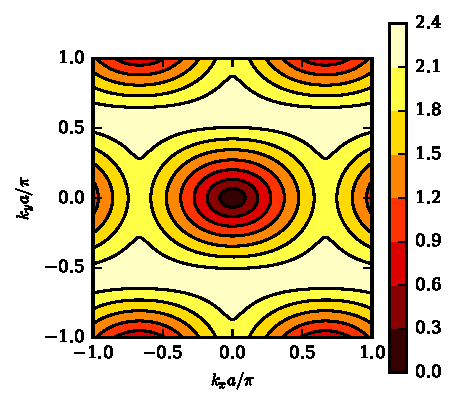
\includegraphics[width=\textwidth]{img/hexagon-disp1.pdf}\caption{First branch.}
        \end{subfigure}\,
%
        \begin{subfigure}[b]{0.49\textwidth}
                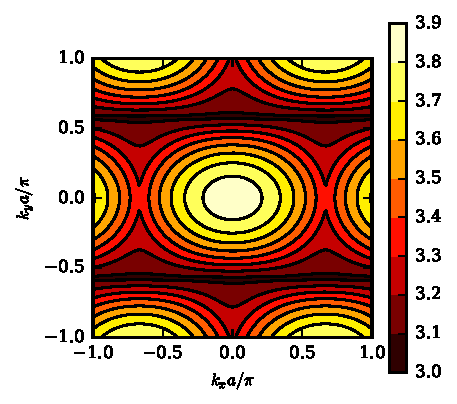
\includegraphics[width=\textwidth]{img/hexagon-disp2.pdf}\caption{Second branch.}
         \end{subfigure}
 \caption{Dispersion relations for the hexagonal unit cell.}\label{fig:hexagon-disp}
\end{figure}

\begin{figure}[h]
  \centering
  \includegraphics[width=4in]{img/{hexagon-irreducible}.pdf}
  \caption{Dispersion curves over the irreducible Brillouin zone.}\label{fig:hexagon-irreducible}
\end{figure}

\end{document}

